\section{Overview}
\label{sec:tofu-overview}

\begin{figure}[t]
\centering
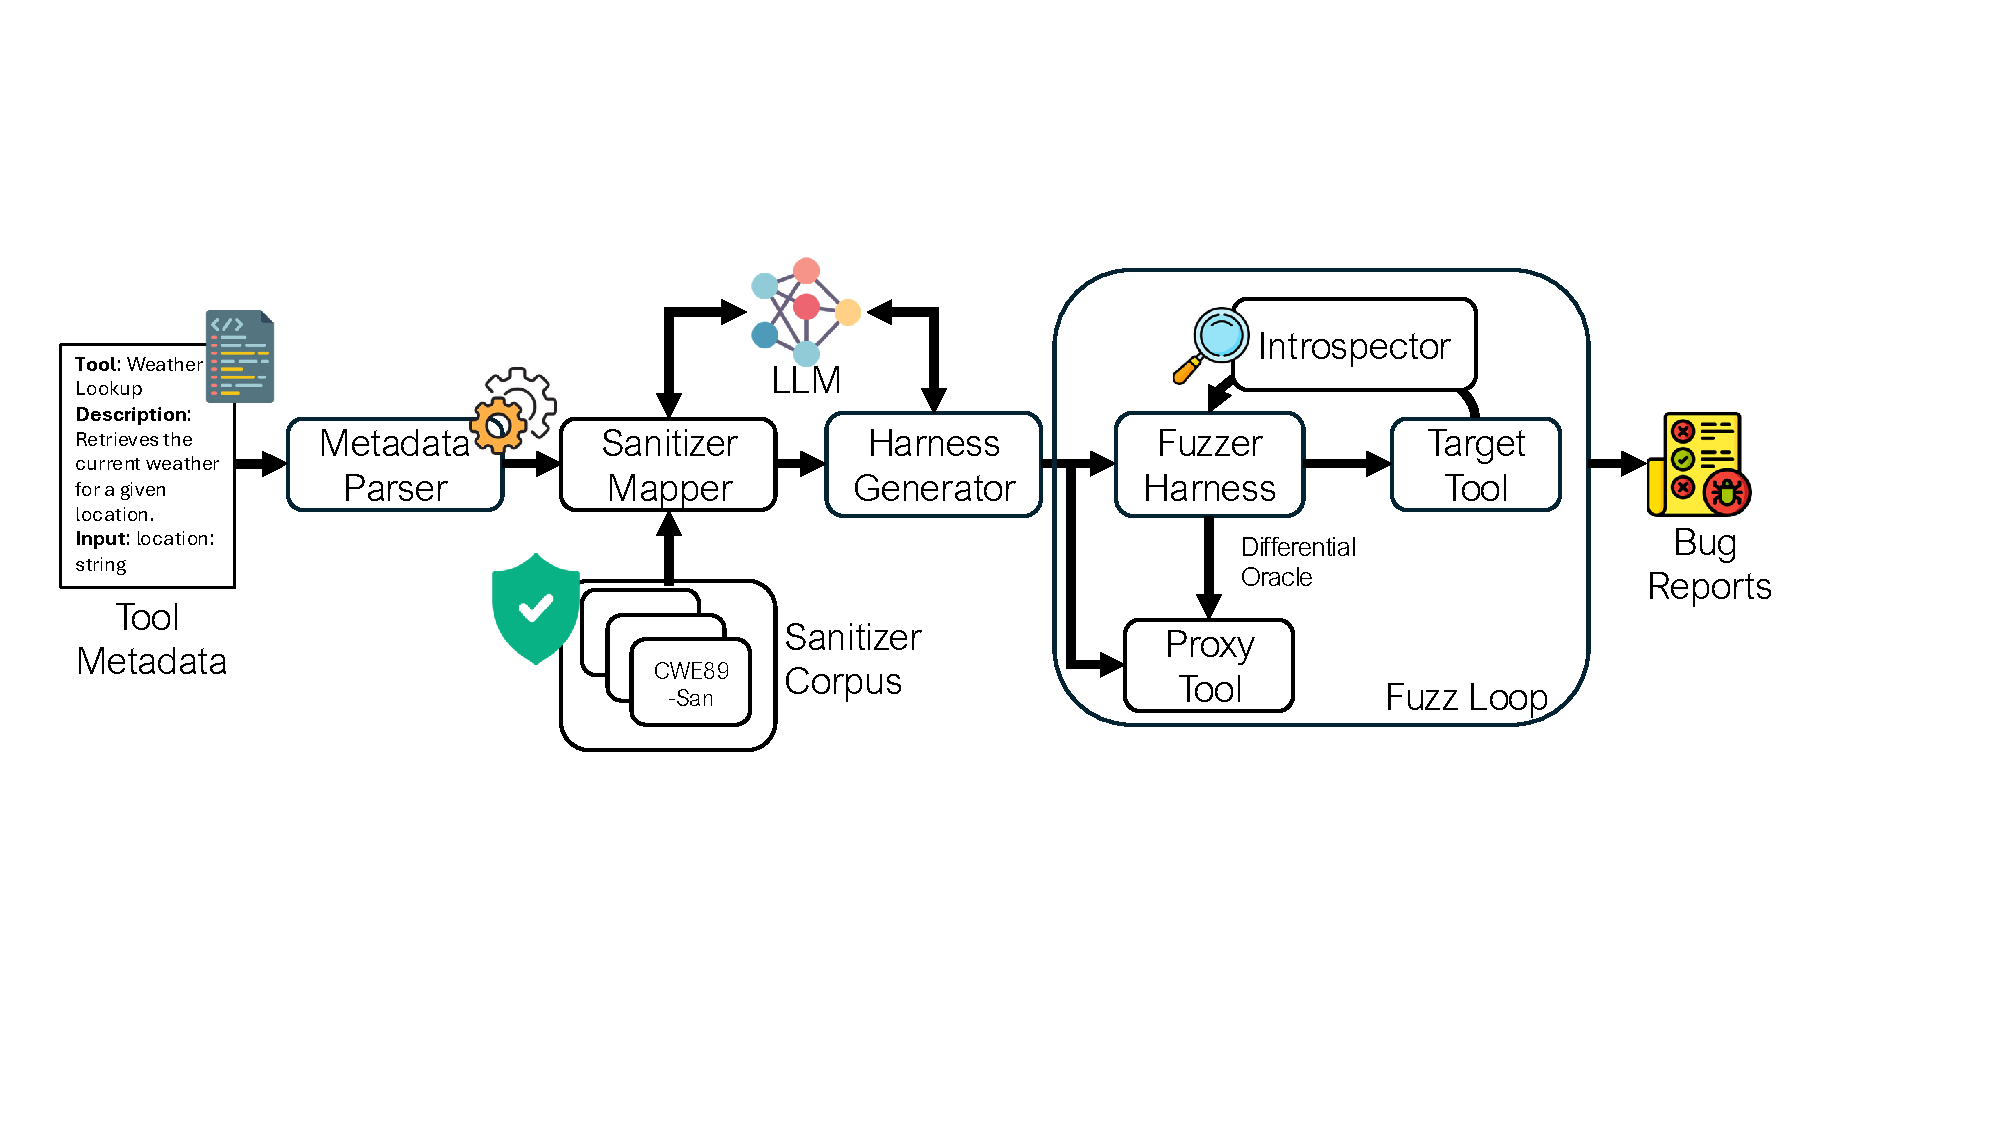
\includegraphics[width=\linewidth]{figs/overview.pdf}
\caption{\project{} maps tool metadata to semantics-aware sanitizers, generates
schema-valid fuzzing harnesses and, when needed, a proxy oracle, and detects
semantic security violations through runtime introspection or differential
checking.}
\Description{Pipeline diagram. A registered tool's metadata enters a Metadata Parser, which feeds a Sanitizer Mapper backed by a CWE-guided Sanitizer Corpus. The resulting specialized security specification drives a Harness Generator, which emits a schema-preserving Fuzzer Harness and, where needed, a Proxy Tool. A Fuzz Loop runs the harness against the target tool and reports violations via either a runtime Introspector or a Differential Oracle.}
\label{fig:tofu-overview}
\end{figure}

\project{} is a tool-aware fuzzing framework that turns the semantic
information already exposed by LLM tools into executable security tests.
As shown in Figure~\ref{fig:tofu-overview}, \project{} takes a registered
tool as input and automatically derives three artifacts: the security
properties to test, a harness that exercises those properties, and an oracle
that determines whether they are violated. \project{} operates through the
tool's existing orchestration interface, reusing its metadata discovery and
invocation mechanisms without requiring changes to the LLM or target tool.

The \textbf{Metadata Parser} first normalizes the tool description, argument
schemas, and natural-language argument descriptions. The \textbf{Sanitizer
Mapper} uses this information to associate each argument with applicable
checks from a CWE-guided \textbf{Sanitizer Corpus}. Each sanitizer couples a
semantic input class with adversarial inputs, an expected security property,
and the observations needed to establish a violation. For example, a path
argument can induce containment and traversal checks, while a URL can induce
scheme and destination checks. An LLM assists in mapping and specializing
these generic sanitizers to the semantics documented by the tool, but the
resulting sanitizer, rather than the LLM, defines the security oracle.

The specialized security specification drives the \textbf{Harness Generator}.
It constructs a \textbf{Fuzzer Harness} that mutates arguments while
preserving the target's schema, allowing adversarial values to traverse the
normal orchestration path and reach the implementation. For targets where
internal behavior cannot be observed, the generator additionally constructs a
\textbf{Proxy Tool} that encodes the expected behavior of the specialized
security checks. Thus, the same semantic specification determines both what
inputs are generated and what behavior is considered secure.

Finally, the \textbf{Fuzz Loop} executes generated invocations against the \textbf{Target Tool}. When implementation-level visibility is available, the \textbf{Introspector} observes sanitizer-relevant effects, such as filesystem, process, or network operations, and directly checks the corresponding property. Otherwise, the \textbf{Differential Oracle} compares the target against the generated proxy and identifies cases where the target accepts or processes an input that violates the inferred contract. Crashes and unhandled failures provide additional feedback. When a violation is detected, \project{} reports the triggering invocation, affected argument, expected property, and observed behavior. Section~\ref{sec:design} describes each stage in detail.
